\documentclass[journal]{IEEEtran}
\usepackage{amsmath,amssymb,bm,graphicx,booktabs,array,cite}
\usepackage{xcolor}
\usepackage[colorlinks=true,linkcolor=blue!50!black,citecolor=blue!50!black,urlcolor=blue!50!black]{hyperref}
\newcommand{\vect}[1]{\boldsymbol{#1}}
\graphicspath{{figures/}}

\begin{document}
\title{Learning the Model Error of a Quadrotor After Complete Rotor Loss: Residual Koopman Model Predictive Control}
\author{Pranshu Kumar, Mudita Jain, Prashant Gupta and Aarush Singh Kushwaha%
\thanks{EE650, Basics of Modern Control Systems. All results are from simulation; code and result tables are in the project repository.}}
\maketitle

\begin{abstract}
After a quadrotor loses one rotor completely it can still fly if it gives up its heading and spins about a tilted axis (the \emph{relaxed hover}). The physics model of this state is good but not exact. We ask whether a Koopman (EDMD) model of only the one-step \emph{error} of the physics model can predict and control the failed drone better than the physics model alone or a Koopman model of the full dynamics. On the plant it was trained on, the residual model is the most accurate predictor from 100\,ms to 1\,s (normalized error 0.64 at 1\,s against 0.91 and 7.09), and ten training episodes suffice to beat the full-state model trained on forty. Inside a convex MPC it reduces a steady altitude error by about one third, but it does not transfer to a plant with different parameters: online adaptation halves the error on the unseen plant and does not help on the training plant, training on capture transients improves the prediction of transients but worsens the capture, and noisy training data are harmful. An LQR with an integrator removes the steady error to at most 0.024\,m and keeps the capture performance, so it is the better remedy. An MPC on the full-state Koopman model is stable near the hover but fails the capture earlier. The conclusions hold on plants with air-relative thrust and quadratic drag.
\end{abstract}

\begin{IEEEkeywords}
fault-tolerant control, quadrotor, rotor failure, Koopman operator, model predictive control, residual learning
\end{IEEEkeywords}

\section{Introduction}
A quadrotor has four thrust inputs for four degrees of freedom, so it has no spare actuator. Mueller and D'Andrea~\cite{mueller2014stability,mueller2016relaxed} showed that after the complete loss of one rotor the vehicle can hold a steady spinning flight, the relaxed hover, and be controlled there by a linear controller on a reduced-attitude model. Their physics model describes the main motion well but misses real effects: less thrust at high spin rate, a spin 20 to 27\% slower than predicted, and uncertain inertia and motor speed. A controller built on it settles with a steady error.

We ask whether a Koopman model of only the one-step error of the physics model~\cite{williams2015edmd,korda2018linear,todde2026residual}, used inside MPC, predicts and controls the failed vehicle better than the physics model alone or than a Koopman model of the full dynamics. Our hypotheses were: (H1) the full-state Koopman model is unstable and loses to a ``no change'' predictor at long horizons; (H2) the residual model predicts best; (H3) the residual MPC removes the steady error; (H4) the residual model needs less data.

\textbf{Contributions.} A controlled comparison of physics-only, full-state Koopman and residual Koopman predictors and MPCs for the failed vehicle, against offset-free and integral baselines, with online adaptation, transient training data, MPC tuning, ablations and a more realistic truth plant. We state novelty only as the outcome of our search (Section~\ref{sec:related}).

\section{Related work}\label{sec:related}
\emph{Control after rotor loss:} feedback linearization and $H_\infty$ loop shaping at a spinning working point~\cite{freddi2011feedback,lanzon2014flight}, LPV control scheduled on the yaw rate~\cite{stephan2018lpv}, upset recovery by control allocation~\cite{sun2020upset}, NMPC~\cite{nan2022nmpc}, and passive schemes without detection~\cite{ke2023uniform}. \emph{Koopman and residual learning:} EDMD with control~\cite{korda2018linear}, residual Koopman MPC for healthy quadrotors~\cite{todde2026residual}, and offset-free Koopman MPC for other systems~\cite{schimperna2025offsetfree}. Some of these papers~\cite{stephan2018lpv,lanzon2014flight} were available to us only as abstracts, so statements about them rely on those. We did not find residual Koopman models in the complete-rotor-loss regime, nor a comparison of offset-free control with a learned residual on a quadrotor.

\section{Model, plants and validation}
The simulator integrates the 6-DOF rigid body with quaternion attitude, gyroscopic terms, per-rotor thrust limits of 0.2 to 3.8\,N and a first-order motor lag (15\,ms). The failed vehicle is described by the reduced attitude $\vect n = R^\top\vect e_3$ with state $(p,q,r,n_x,n_y,z,v_z)$ and three motor states; its relaxed hover (thrusts $(2.04, 1.02, 2.04, 0)$\,N, body rates $(0, 5.37, 18.8)$\,rad/s) is a fixed point of these coordinates, so its linearization is time-invariant. The simulator reproduces the published two- and three-rotor-loss equilibria to every printed digit, five hover solutions of the IJRR model within 4\%, and the flight spin-up time within about 4\%. For learning, \emph{truth plants} add effects the nominal model lacks: thrust loss at high body rate, inertia errors and slower motors (family A for training, family B held out); families A$^+$ and B$^+$ add air-relative thrust and quadratic drag.

\subsection{Capture protocol}
At $t=0$ rotor 4 fails and the healthy LQR keeps flying for a detection delay $\tau$; then rotors 1 and 3 run at 2.95\,N with rotor 2 stopped and no feedback until the body rate exceeds 10\,rad/s, when the failure LQR or MPC takes over. A run is \emph{safe} if the attitude is captured over the last second, the height loss is below 2\,m and the drone never turns over (criterion fixed in the code before the runs). The LQR is safe for delays up to about 10\,ms.

\section{Predictors and prediction results}
Data are closed-loop episodes of the failure LQR with random excitation on the truth plant (40 episodes of 4\,s at 5\,ms; test: 10 episodes each of A and B). The \emph{analytical} predictor is the 10-state linear model. The \emph{full-state EDMDc} uses 55 functions (constant, 9 standardized states and filtered commands, all degree-2 monomials). The \emph{residual EDMDc} adds to the analytical one-step prediction a learned correction $W^\top\psi$ (91 functions, ridge, clipped at the 99.5\% percentile of the training residuals).

\begin{figure}[t]
\centering
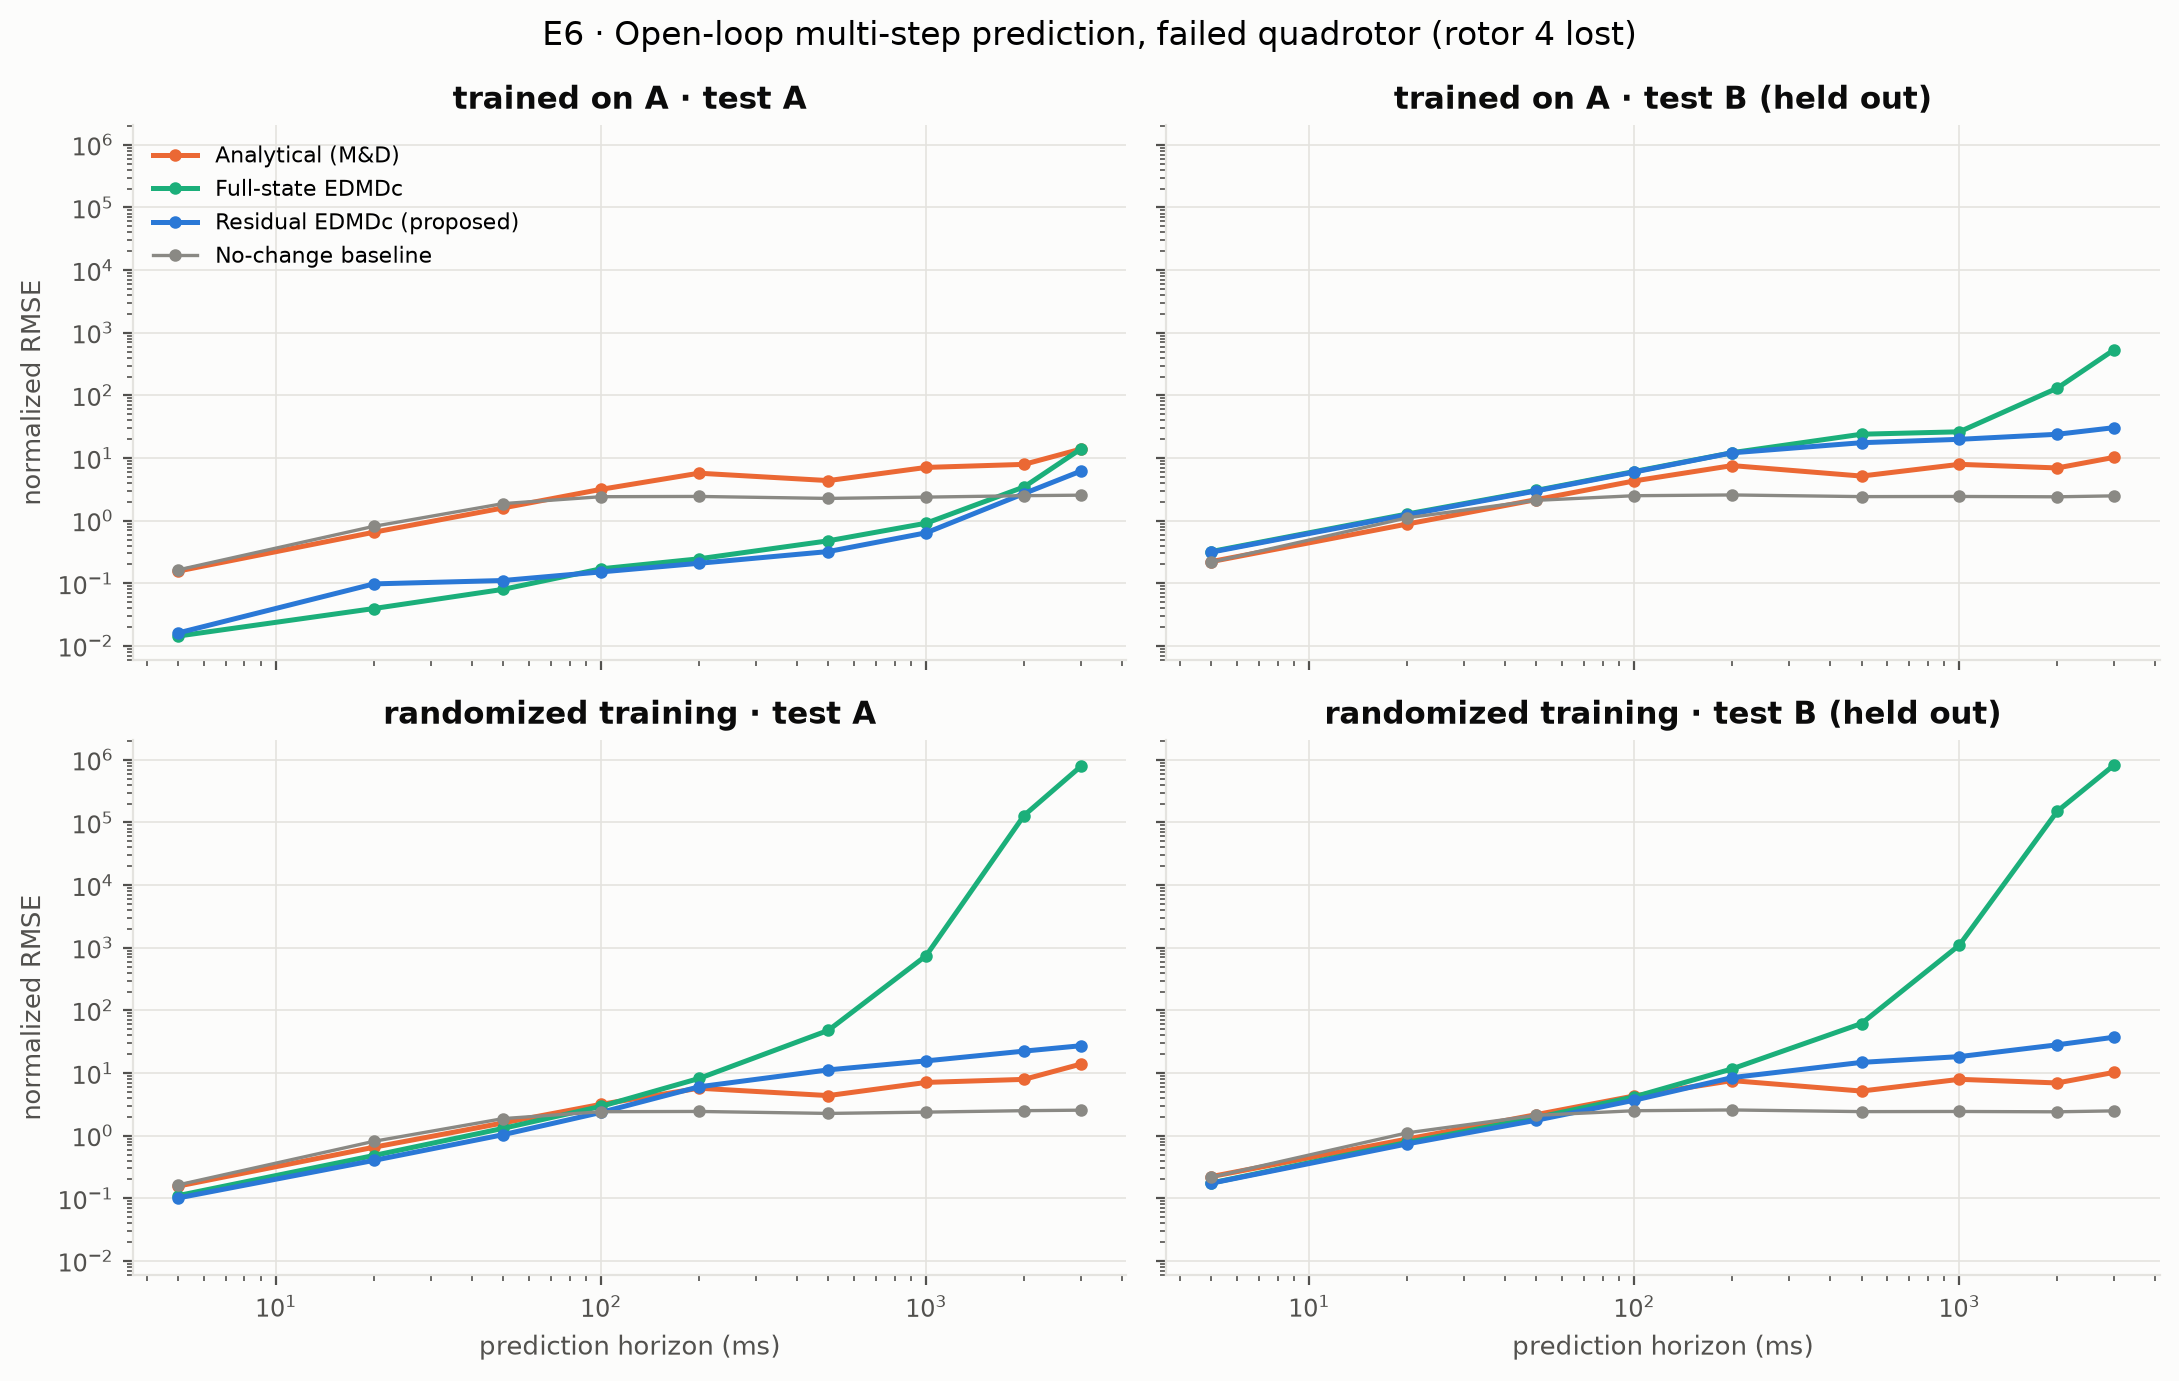
\includegraphics[width=\linewidth]{e6_multistep_error.png}
\caption{Multi-step prediction error against horizon (normalized RMSE), four settings.}\label{fig:e6}
\end{figure}

The residual model is the most accurate from 100\,ms to 1\,s on the training plant (Fig.~\ref{fig:e6}; 1\,s error 0.64, against 0.91 for the full-state and 7.09 for the analytical model), and 10 episodes suffice to beat the full-state model trained on 40. The full-state operator has 4 of 55 eigenvalues outside the unit circle (spectral radius 1.007) and falls behind a ``no change'' predictor by 2\,s. On the held-out family B all learned models are worse than the analytical model at short horizons (100\,ms: 5.9 for the residual against 4.3), so the residual behaves as a calibration of one vehicle.

\section{MPC and baselines}
\begin{figure}[t]
\centering
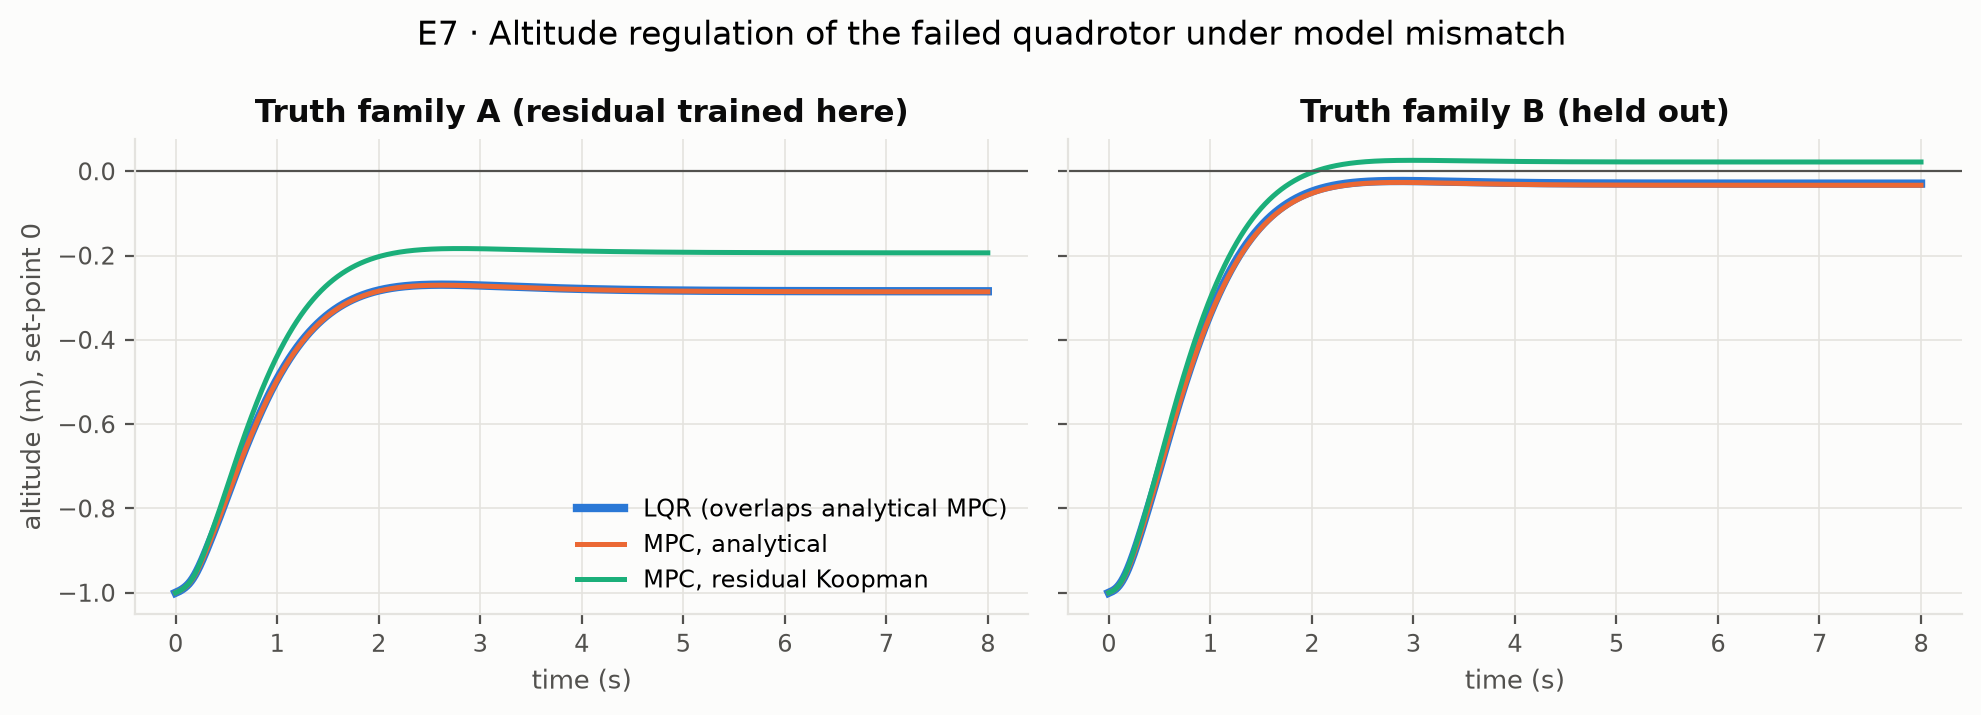
\includegraphics[width=\linewidth]{e7_altitude.png}
\caption{Altitude under model mismatch: LQR, analytical MPC and residual MPC (families A and B).}\label{fig:e7}
\end{figure}

The MPC (horizon 20, DARE terminal cost, thrust limits, OSQP) treats the residual as a constant measured disturbance outside the QP. Near the hover the steady altitude error is $-0.285$\,m for the LQR, $-0.286$ for the analytical MPC and $-0.193$ for the residual MPC on family A (32\% less), but the residual MPC is worse than the LQR on one held-out variant ($+0.164$ against $+0.112$\,m). An \emph{offset-free} MPC with a disturbance on all physical states removes the bias (0.000\,m on six plants) but fails the capture even at 0\,ms; the first, pre-registered design with three thrust-offset disturbances leaves $-0.239$\,m. An LQR with an integrator on the altitude reduces the bias to at most 0.024\,m \emph{and} keeps the LQR's capture, so it beats the residual MPC on both counts. An MPC on the full-state Koopman model, re-lifted at every step, is stable near the hover with similar errors ($-0.186$\,m on A), but capture fails already at 10\,ms of delay and it needs 55 to 319\,ms per step.

\begin{figure}[t]
\centering
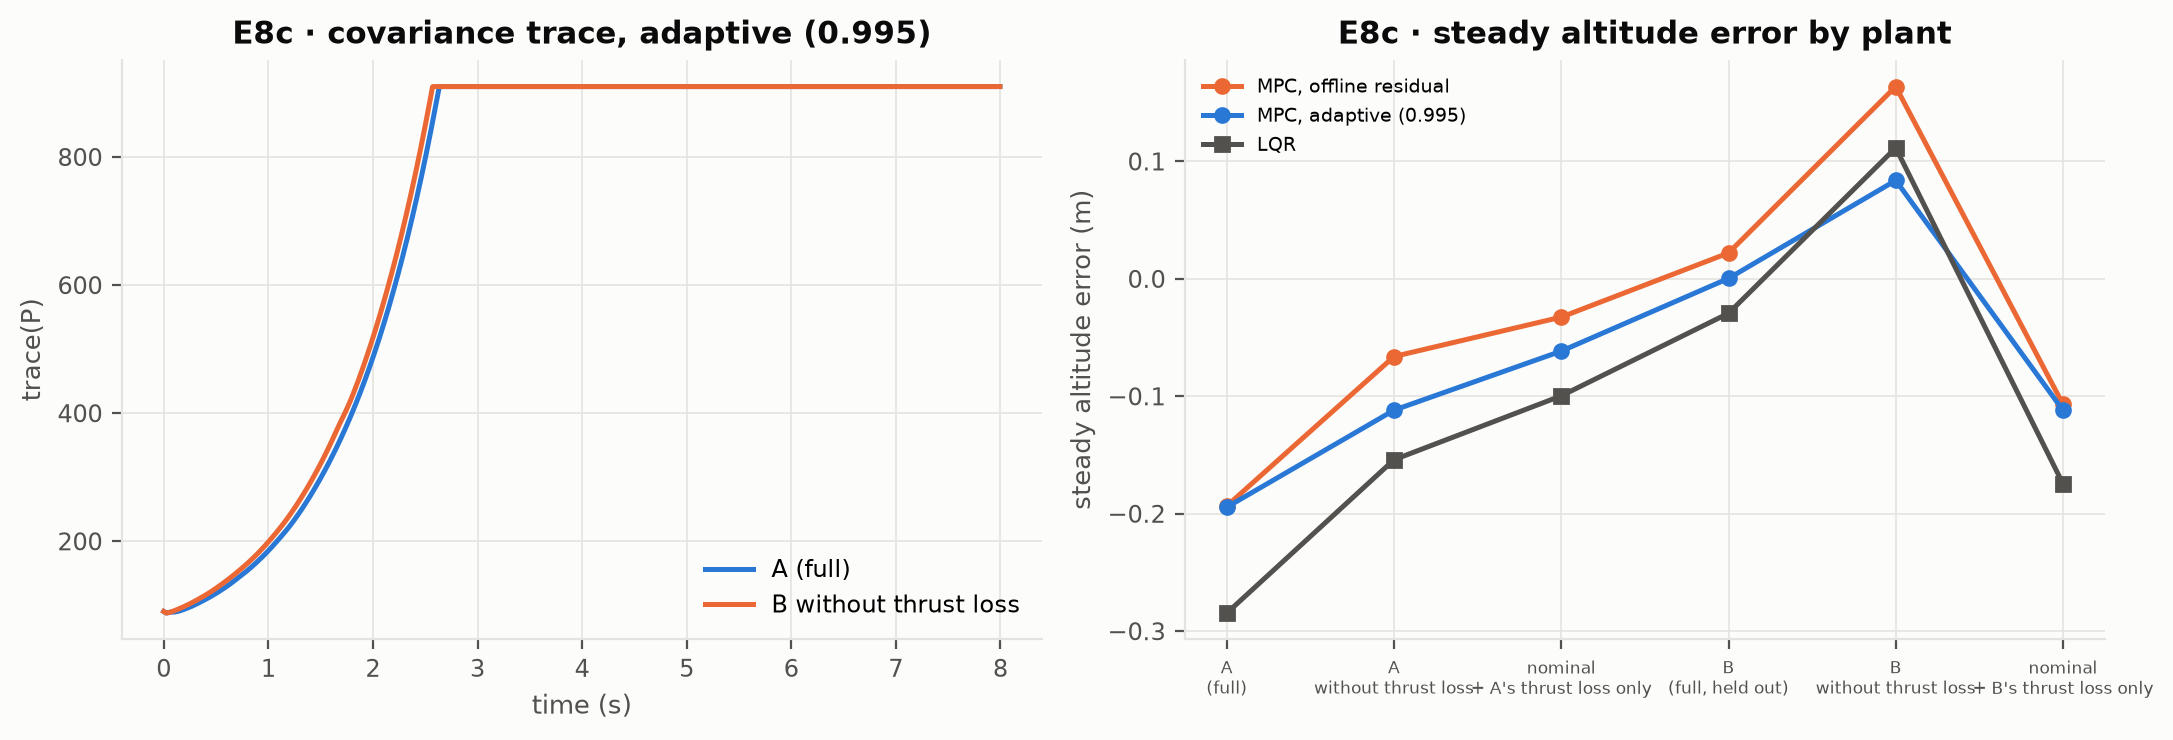
\includegraphics[width=\linewidth]{e8c_adaptive.png}
\caption{Left: covariance trace of the adaptive residual. Right: steady altitude error by plant.}\label{fig:e8c}
\end{figure}

\section{Adaptation, transients, tuning, ablations}
\emph{Online adaptation.} Recursive least squares on the residual weights (forgetting factor 0.995, causal update) halves the prediction error on family B (100\,ms: 2.8 against 5.9) and repairs the worst closed-loop plant ($+0.084$ against $+0.164$\,m, LQR $+0.112$), but is no better on family A (0.5\,s: 1.30 against 0.30), and the covariance guard is saturated (Fig.~\ref{fig:e8c}). \emph{Transient training.} A residual trained on capture transients predicts held-out transients an order of magnitude better (100\,ms: 0.57 against 8.2) but the MPC built on it is not safe even at 0\,ms. \emph{MPC tuning.} Horizons from 10 to 80 steps do not change the number of safe delays and a heavier attitude weight adds one, equalling but not exceeding the LQR; horizon 80 needs 84 to 123\,ms per step. \emph{Ablations.} Cubic features reduce the long-horizon error on B (3\,s: 5.9 against 30.6) but are worse on A at 100\,ms; the ridge parameter and the sampling period (2 to 10\,ms) do not matter; training on noisy measurements is harmful (closed-loop bias $+2.8$\,m, errors in the regressors bias the fit) whereas the clean-trained residual and the offset-free MPC tolerate noise. \emph{Realistic plant.} On families A$^+$ and B$^+$ the conclusions are unchanged (LQR $-0.412$\,m, residual MPC $-0.273$, offset-free 0.000, integrator at most 0.018\,m).

\section{Discussion and limitations}
Hypotheses H1 and H4 are supported, H2 on the training plant only, and H3 partly (a third less error on the training plant, worse on one held-out plant). The residual helps near the plant it was trained on, but for removing a steady error integral action is better, and nothing we added to make the residual more general or more capable improved the capture. Limitations: simulation only on our own simulator; the recovery strategy was reimplemented from the paper and its spin-up thrust was read from a plot; all controllers are given the exact state; learning data are recorded under feedback; one vehicle; and some closely related papers were available only as abstracts.

\section{Conclusion}
Learning only the error of the physics model gives the best predictions from 100\,ms to 1\,s on the plant it was trained on and removes a third of a steady altitude error inside a convex MPC, but it does not carry over to other plants, an integral controller removes the error better, and no learned variant tested improved the capture after a detection delay. Grey-box estimation of the uncertain physical parameters, a state estimator and hardware tests are the next steps.

\bibliographystyle{IEEEtran}
\bibliography{../report/references}
\end{document}
